% !TEX root = ../HPCA2016.tex
\section{Introduction}
\label{sec:Introduction}

In recent years improvement of system performance has been impeded by the memory wall problem ~\cite{wulf-can95}. To alleviate the memory wall problem there has been a lot of recent research in the use of 3-D die-stacked memory to provide high performance. Placing 3D memory stacks in the same package as the processor can provide significant improvements in bandwidth and lower power consumption ~\cite{black-micro2013}.  There has 
has been significant advancement in the industry including the development of
die-stacked memory standards and consortia~\cite{jedec-wideio,JEDEC-HBM,pawlowski-hotchips2011},
and various announcements from several processor
companies~\cite{KnightsLanding,NVIDIA,black-micro2013}.

Current stacking technology may provide on the order of eight 3D DRAM stacks, each with 2GB capacity, for a total of 16GB of
fast DRAM~\cite{KnightsLanding}.  However, many server systems already support
{\em hundreds} of GB of memory and so a few tens will not suffice for the
problem sizes and workloads of interest.  The resulting system will therefore
consist of two types of memory: a first class of fast, in-package, die-stacked
memory, and a second class of off-package commodity memory (e.g., double data rate type 3 (DDR3)).

Given such a {\em Two-Level Memory} (TLM) hybrid memory organization, the challenge then
comes from determining how to best organize and manage this system. The goal of any management is to give the performance of the fast in-package memory while still providing the capacity of the larger off-package memory. 
A large body of recent body of recent research has focused on utilizing the stacked DRAM as a
large, high-bandwidth last-level cache (e.g., an ``L4'' cache), coping with the
challenges of managing the large tag storage required and the relatively slower
latencies of DRAM (compared to on-chip SRAM)~\cite{loh-micro2011,qureshi-micro2012,jevdjic-isca2013,jiang-hpca2010,zhao-iccd2007,sim-micro2012,meza-cal2012,elnacouzi-date2013,hameed-cases2013}.  
Such a hardware caching approach has some immediate advantages, especially that of
software-transparency and backwards compatibility.  As the stacked DRAM is
simply another cache that is transparent to the software layers, any existing
applications can be run on a system with such a DRAM cache and potentially
obtain performance and/or energy benefits~\cite{loh-shaw2012}. 
One drawback of the caching approach is that stacked memory is not available for application use. While the capacities of die-stacked memory is likely to be insufficient to serve as the entirety of a system's main memory it is still non-trivial in size and would be beneficial to memory capacity constrained workloads ~\cite{chou-micro2014}.

An alternative configuration is to expose the die-stacked memory as part of the main memory capacity. In this configuration the management and efficient use of the TLM hybrid memory lies on the application and the underlying management option. One recent research explored  management by the operating system (OS) ~\cite{meswani-hpca21}. The OS monitors memory usage and periodically performs page migrations to move frequently accessed pages to stacked memory. 
One of the many challenges that OS or any runtime implementation faces is that it is constrained by the overheads of management. The OS needs to take an interrupt to do anything, additionally the OS then has to traverse the page tables to read the access frequency information,  migrate pages and update the page table entries to reflect the change of virtual to physical address mapping and flush the translation lookaside buffers (TLB). As we show in our evaluations, these costs are non-trivial and constraint the OS to set the minimum management intervals or epochs to 0.1 seconds. Such coarse grained intervals leaves a lot of opportunities on the table. 

Most recently ~\cite{sim-micro2014} proposed a transparent hardware schem to manage TLM as a flat address space. The main contributions of that work was the use of storage efficient structures to track page access frequency and remapping tables. They allow migrations to happen between any aribitrary channels and the use of single centralized migrator can become a bottleneck when systems scale to terabytes of memory and 10s of channels. To this end we in this paper we introduce  the migration cluster architecture that is specifically designed to scale to systems of future. Our migration clusters group channels of different memory levels into smaller cluster sets and migration is limited to within cluster only. In this clustered architecture we also use page access counting hardware that can store information for millions of pages as well as we use remap tables that can remap millions of pages in the cluster efficiently. We also describe and evaluate novel migration algorithms that are able to optimize for latency and bandwidth sensistive workloads in a CPU-GPU system. 

\begin{figure}[h]
  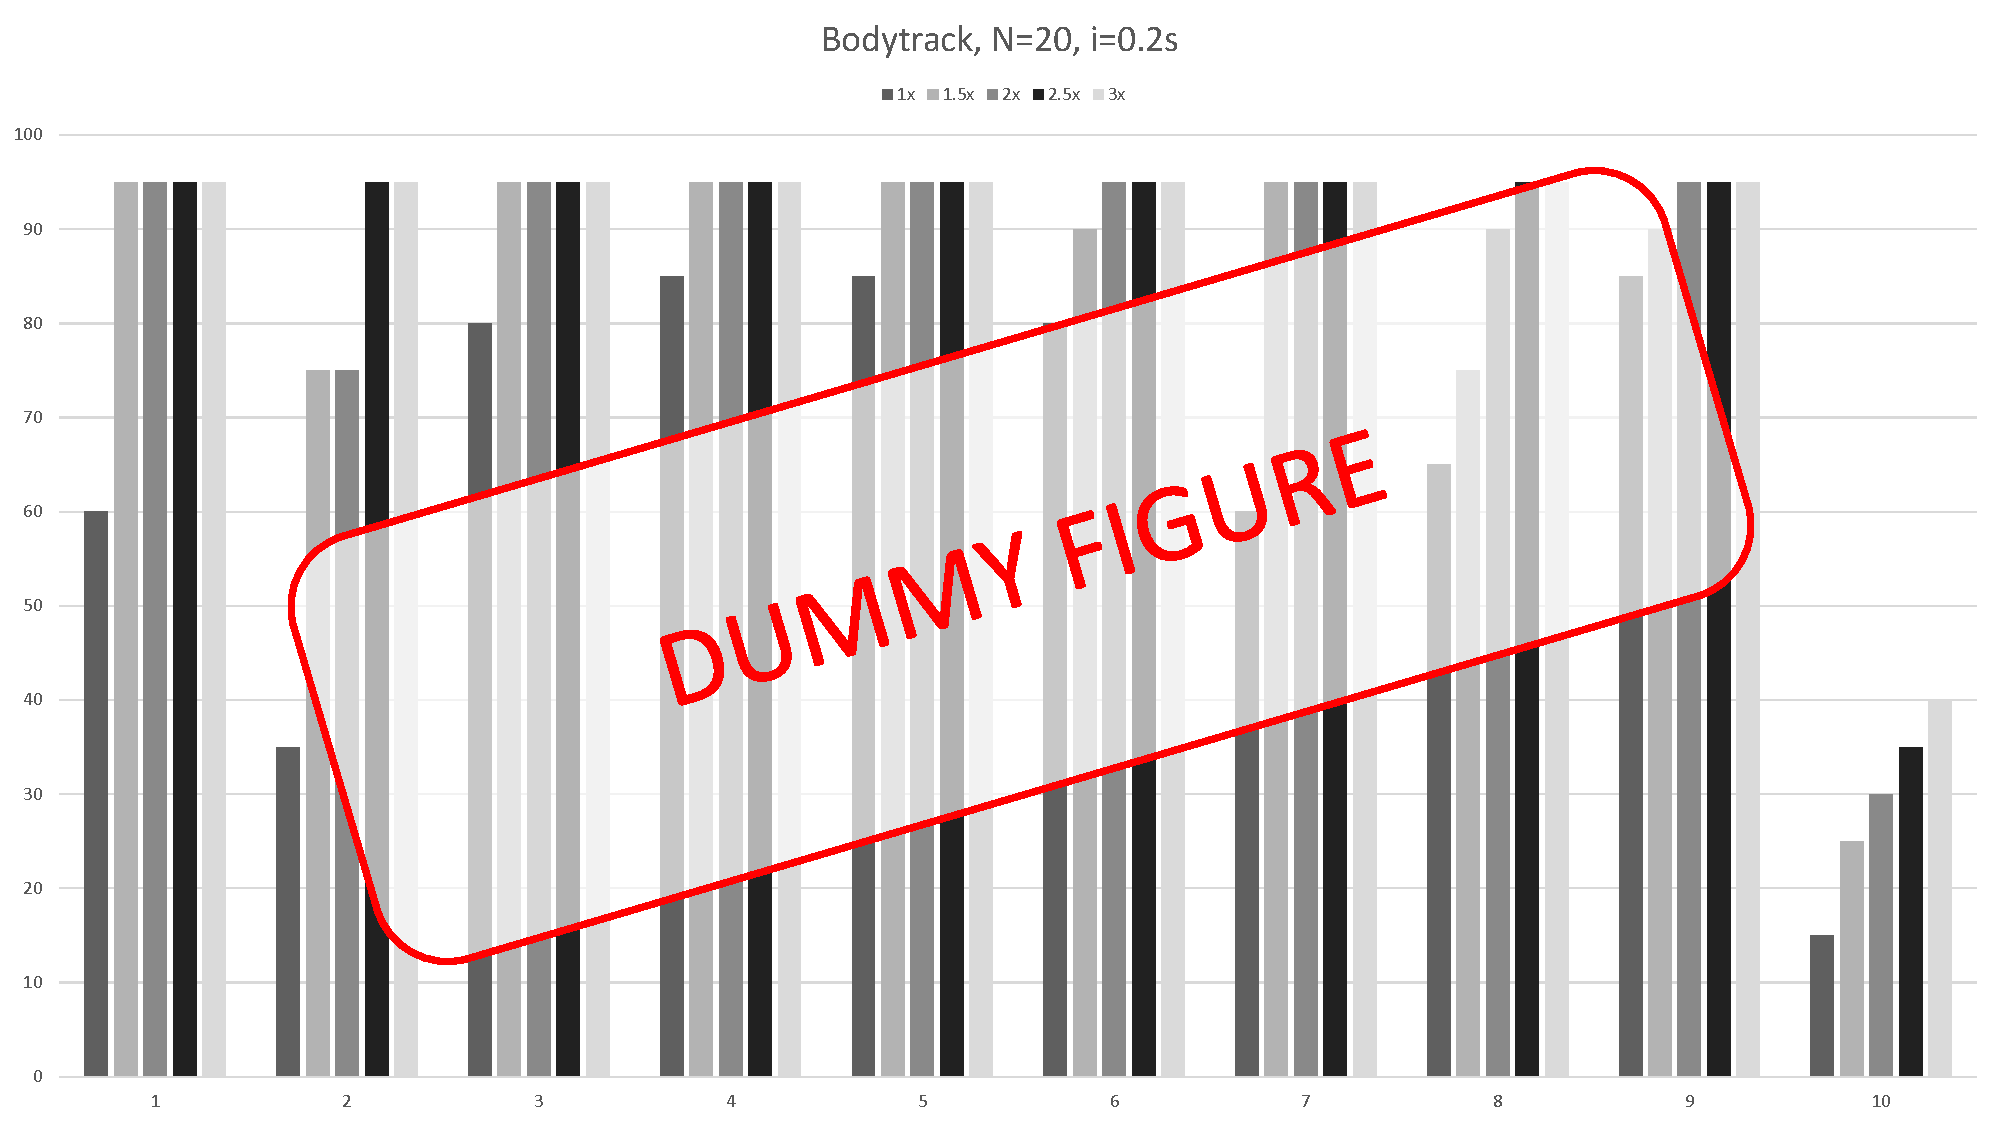
\includegraphics[width=0.46\textwidth]{figures/dummy.pdf}
  \caption{Dummy figure caption 2}
  \label{fig:dummy2}
\end{figure}





Show graph with motivational result.

List the paper's main contributions.

Overview of paper's chapters.
